
\documentclass[12pt, a4paper]{article}

%-----------USEPACKAGE----------------------------
\usepackage{bm} % Tucne pismo
\usepackage[czech]{babel} % Cestina
\usepackage[T1]{fontenc}
\usepackage[utf8x]{inputenc}
\linespread{1.10} % Radkovani 1.3 odpovida radkovani 2
\usepackage{lmodern} % Daji se pouzit \HUGE atd.
\usepackage{amsmath}
\usepackage{algorithm}
\usepackage[noend]{algpseudocode} % Vkladani pseudo kodu
\usepackage{listings}
\usepackage{setspace}

% Graphics
\usepackage{graphicx}
\usepackage{epstopdf}
\usepackage{color}
\graphicspath{{./img/}}

% Hyperref and its color
\usepackage[unicode]{hyperref} % Odkazy v pdf, www a na e-mail
\usepackage[hypcap=true]{caption}
\usepackage[hypcap=true,list=true]{subcaption}
\hypersetup{colorlinks = true, citecolor = black}
\hypersetup{linkcolor=red}
\hypersetup{colorlinks,urlcolor=black}






%-----------COLORS--------------------------------
\definecolor{Code}{rgb}{0,0,0}
\definecolor{Decorators}{rgb}{0.5,0.5,0.5}
\definecolor{Numbers}{rgb}{0.5,0,0}
\definecolor{MatchingBrackets}{rgb}{0.25,0.5,0.5}
\definecolor{Keywords}{rgb}{0,0,1}
\definecolor{self}{rgb}{0,0,0}
\definecolor{Strings}{rgb}{0,0.63,0}
\definecolor{Comments}{rgb}{0,0.63,1}
\definecolor{Backquotes}{rgb}{0,0,0}
\definecolor{Classname}{rgb}{0,0,0}
\definecolor{FunctionName}{rgb}{0,0,0}
\definecolor{Operators}{rgb}{0,0,0}
\definecolor{Background}{rgb}{1, 1, 1}

%-----------LISTINGS-SETTINGS----------------------
\lstset{
	numbers=left,
	numberstyle=\footnotesize,
	numbersep=0.5em,
	xleftmargin=1.5em,
	xrightmargin=0em,
	framextopmargin=0em,
	framexbottommargin=0em,
	showspaces=false,
	showtabs=false,
	showstringspaces=false,
	frame=lrtb,
	tabsize=4,
	% Basic
	basicstyle=\ttfamily\footnotesize\setstretch{1},
	backgroundcolor=\color{Background},
	language=Python,
	% Comments
	commentstyle=\color{Comments}\slshape,
	% Strings
	stringstyle=\color{Strings},
	morecomment=[s][\color{Strings}]{"""}{"""},
	morecomment=[s][\color{Strings}]{'''}{'''},
	% Keywords
morekeywords={import,from,class,def,for,while,if,is,in,elif,else,not,and,or,print,break,continue,return,True,False,None,access,as,del,except,exec,finally,global,import,lambda,pass,print,raise,try,assert},
	keywordstyle={\color{Keywords}\bfseries},
	% Additional keywords
	morekeywords={[2]@invariant},
	keywordstyle={[2]\color{Decorators}\slshape},
	emph={self},
	emphstyle={\color{self}\slshape},
	breaklines=true, % Zalamuje radky.
}






%------------------VARIABLES----------------------------
\newcommand{\cisloCviceni}{8. cvičení}









%------------------LAYOUT----------------------------
\usepackage[top = 2.5 cm, bottom = 2.5 cm, left = 2.5 cm, right = 2.5 cm]{geometry} % geometrie stranky
\usepackage{longtable}% Pro dlouhy obsah, da se zalomit \pagebrek
\usepackage{fancyhdr}
\pagestyle{fancy}% Deffaultni nastaveni hlavicky a paticky
\setlength{\headheight}{16 pt}% Zvetsi hlavicku, aby to nedelalo warningy
\fancyhf{}
\lhead{\href{http://www.kky.zcu.cz/cs/courses/mpv}{Metody Počítačového Vidění}}
\rhead{\cisloCviceni}
\fancyfoot[R]{\thepage}
\fancyfoot[L]{Verze 2.0.0, poslední úpravy: \today}








%---------------BEGIN-DOCUMENT--------------------------
\begin{document}
 









 
%--------TITLE-PAGE--------------------------------------------
\begin{titlepage}
\begin{center}
	
\includegraphics[trim = 0.6cm 0.5cm 0.9cm 0.5cm, scale=1]{./FAV_logo_cz.pdf}
	\hspace*{\fill}
	
\includegraphics[trim = 3.5cm 1.5cm 2.6cm 2cm, scale=0.295]{./KKY_logo_cz.pdf}\\
	\vspace*{\fill}
	\textbf{\Huge{\href{http://www.kky.zcu.cz/cs/courses/mpv}{Metody Počítačového Vidění} \\ ~ \\ \cisloCviceni}}\\
	\vspace*{\fill}
	\textbf{\large{\href{mailto:LBures@kky.zcu.cz}{Ing. Lukáš Bureš}}} \hfill \textbf{\large{Plzeň, \today}}
\end{center}
\end{titlepage}












%--------OBSAH-CVICENI---------------------------------
\section*{Obsah cvičení}
\begin{enumerate}
	\item Klasifikace
	\item Recall, Precision, F1 score
\end{enumerate}








%-------------------------------------------------------------------------------
\section{Klasifikace}
\par{Ve strojovém učení a statistice je klasifikace problém identifikace, ke kterému ze souboru kategorií patří nová pozorování a to na základě trénovací množiny dat. Příkladem by mohl být antispamový filtr, který na základě jména klasifikuje do složek \uv{je spam} nebo \uv{není spam}.}

\par{V terminologii strojového učení je klasifikace za instanci učení s učitelem, tj učení, kde je k dispozici trénovací sada správně označených pozorování. Podobně, klasifikaci, kde není informace od učitele se říká shlukování a zahrnuje seskupování dat do kategorií na základě jisté míry přirozené podobnosti nebo vzdálenosti.}

\par{Často mají jednotlivá pozorování sadu měřitelných vlastností. Tyto vlastnosti mohou představovat jednotlivé kategorie například typ krevní skupiny, pořadové číslo (\uv{malé}, \uv{střední}, \uv{velké}.}

\par{Algoritmus, který provádí klasifikaci a to zejména v konkrétním provedení je známý jako klasifikátor. Termín \uv{klasifikátor} někdy také odkazuje na matematické funkce, realizované klasifikačním algoritmem, který mapuje vstupní data do kategorií.}

\par{Terminologie skrze vědecké oblasti je velice pestrá. Ve statistice, kde se klasifikace často provádí binární regresí nebo obdobným postupem se pozorované proměnné nazývají \uv{nezávislé proměnné} a predikované kategorie jsou známé jako výsledky, které je možné považovat za závislé proměnné. Ve strojovém učení jsou pozorování známá jako instance a nezávislé proměnné jsou nazývány příznaky, které se sdružují do příznakových vektorů. Dále jsou kategorie nazývány třídami.}












%-------------------------------------------------------------------------------
%\section{Data, třídy}
%\par{}









\newpage

%-------------------------------------------------------------------------------
\section{Recall, Precision, F1 score}
\par{}

\begin{figure}[!ht]
	\centering
	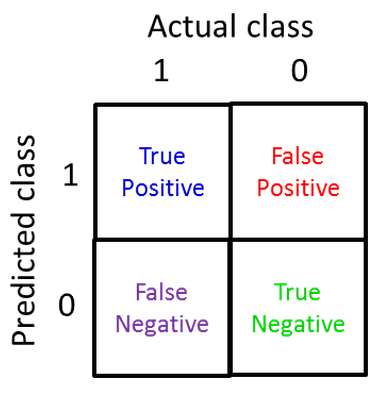
\includegraphics[width = 0.5\textwidth]{Tabulka.png}
\end{figure}


\subsubsection*{Precision}
Precision is the probability that a (randomly selected) retrieved document is relevant.
\begin{equation}
	\mbox{Precision} = \frac{\mbox{True positives}}{\# \mbox{predicted as positive}} = \frac{\mbox{True positives}}{\mbox{True positives + False positives}}
\end{equation}

\subsubsection*{Recall}
Recall is the probability that a (randomly selected) relevant document is retrieved in a~search.
\begin{equation}
	\mbox{Recall} = \frac{\mbox{True positives}}{\# \mbox{actual positives}} = \frac{\mbox{True positives}}{\mbox{True positives + False negatives}}
\end{equation}

\subsubsection*{F1 score}
A measure that combines precision and recall is the harmonic mean of precision and recall.
\begin{equation}
	\mbox{F1 score} = 2 \cdot \frac{\mbox{Precision $\cdot$ Recall}}{\mbox{Precision + Recall}}
\end{equation}

\end{document}



















